\chapter{Resultados}

Neste capítulo é apresenta a ferramenta obtida assim como detalhes sobre o tempo de execução.


\section[Parte Gráfica]{Parte Gráfica}

A parte gráfica da ferramenta é baseada em duas telas, a tela de exibição que se assemelha a um player e é responsavel exclusivamente para exibir o video e suas modificações e o painel de controle que é destacada do player porem sua unica função é controllar o que será exibido no player.


\begin{figure}[H]
	\centering
	\caption{Tela ``player''}
	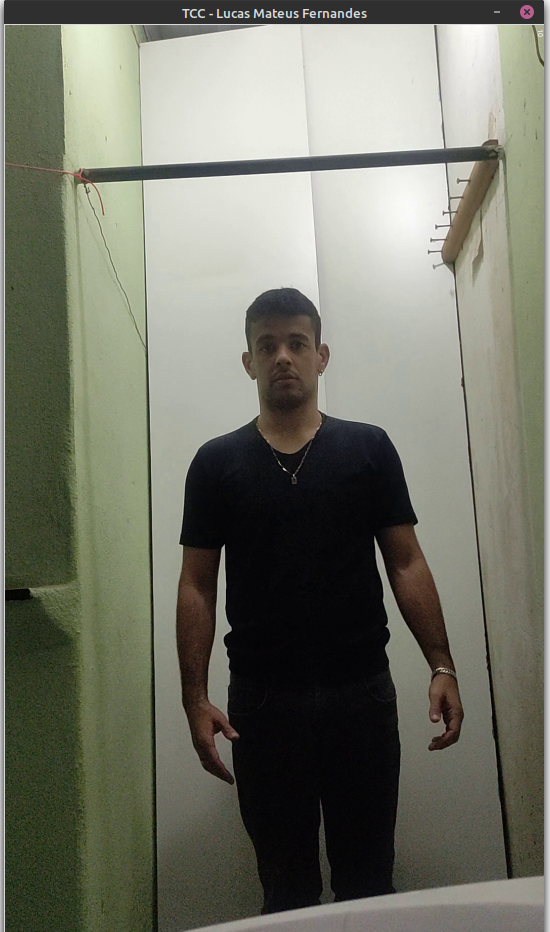
\includegraphics[scale=0.25]{figuras/view/player.png}
	\legend{Fonte: Elaborado pelo autor (2023)}
\end{figure}


A tela responsavel por ser um painel de controle do player possui nove campos de entrada sendo  2 caixas de texto  "Speed" e "Frame" e cinco botões "PLAY", "SaveF", "SaveV", "Barra", "Dados" e "EPH" e uma barra deslizante. 


\begin{figure}[H]
	\centering
	\caption{Tela ``painel de controle''}
	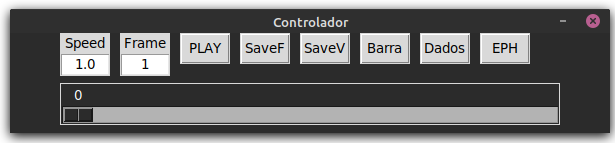
\includegraphics[scale=0.5]{figuras/view/painel_controller.png}
	\legend{Fonte: Elaborado pelo autor (2023)}
\end{figure}

A caixade texto "Speed" recebe como entrada um numero decimal que representa um scalar pelo qual a velocidade de reproduçaõ vai ser alterada. A caixade texto "Frame" recebe como entrada um numero inteiro e faz com que o video se mova para o \textit{frame} semelhante a barra deslizante que altera o frame em exibição. O botão "PLAY" é responsavel por reproduzir o video e pausar. O botão "SaveF" é responsavel por salvar o frame visualizado no diretorio ./midia/dist do projeto analogamente o botão "SaveV" faz o mesmo porem para um video e não uma imagem. O botão "Barra" é responsavel por  destacar a posição da barra no video. O botão "EPH" é responsavel por destacar a pose do executor traçando segmento de retas sobre os membros e o tronco. O botão "Dados" é responsavel por exibir no canto esquerdo superior informações como  
 id do frame, o estado do \ac{AFD} a quantidade de barras realizada, o angulo entre o braço e ante braço, o angulo formado pela perna e coxa, o angulo pelo qual o video teve que ser rotacionado para a barra ficar paralela ao solo, condiçoes como, se a mão esta tocando a barra se o cotovelo esta extendido ou flexionado se as pernas estão dobradas, se a cabeça ultrapassou a barra, a distancia do peito até a barra, se o peito tocou a barra e o caracter do \ac{AFD} que representa o frame atual.


\begin{figure}[H]
	\centering
	\caption{Resultado final com todas as Flags ativas ``Barra'',``Dados'' e ``EPH''}
	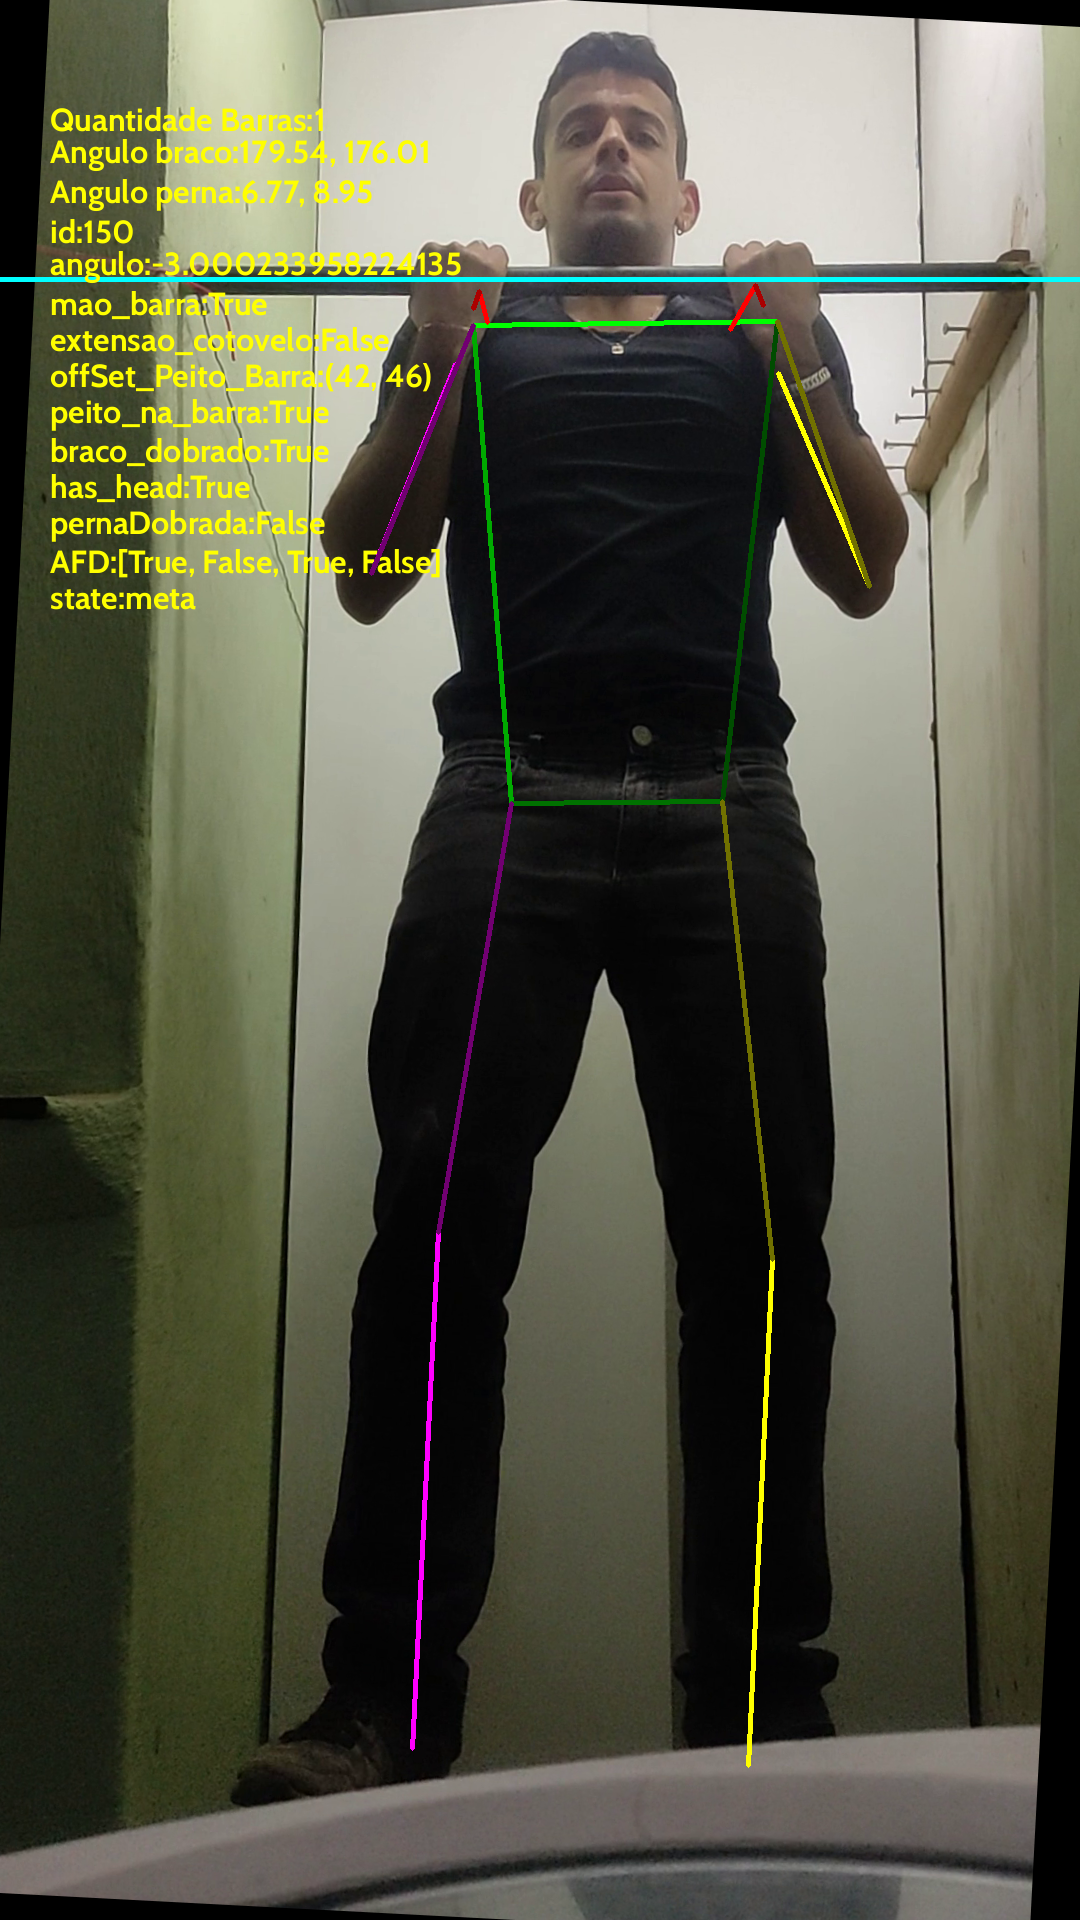
\includegraphics[scale=0.2]{figuras/flags.png}
	\legend{Fonte: Elaborado pelo autor (2023)}
\end{figure}



\section[Tempo de execução]{Tempo de execução}

O tempo de execução desempenha um papel crucial pois representa o intervalo de tempo necessário para que um programa ou algoritmo conclua uma tarefa específica e é um fator fundamental na avaliação e otimização de sistemas computacionais utilizado como métrica para comparar a eficiência de diferentes abordagens e soluções, buscando identificar a estratégia mais eficaz para realizar uma tarefa determinada.Portanto para os testes foi avaliado um video de 211 frames a uma taxa de 24 frames por segundos realizando um execução correta do movimento de barra fixa, para a amostragem foi realizado 10 iterações da execução o programa.


\newpage
Para um melhor entendimento dos resultados o processamento de um frame foi denominado de 'process\_cell' e é subdividido em funções sendo elas:


\begin{itemize}
	\item Função barra responsável pela Detecção da barra, conforme demonstrado na seção \ref{sec:Deteccao da barra}.

	\item Função verify\_inclination responsável pela rotação da imagem de acordo com a inclinação da barra, conforme demonstrado na seção \ref{sec:Inclinacao da barra}.

	\item Função verify\_eph responsável pela identificação dos pontos chaves do corpo humano, conforme demonstrado na seção \ref{sec:Reconhecimento de pose humana}.

	\item Função verify\_angle\_member responsável pela identificação dos angulos entre os segmentos, conforme demonstrado na seção \ref{angulo_braco} e \ref{sec:Movimentacao do quadril}. 

	\item Função verify\_char\_AFD responsavel pela extração das informações presente no caracter do \ac{AFD} conforme explicado em \ref{sec:Estrategia para deteccao do movimento correto de barra fixa} Sendo um compilado de 4 funções 
	
	\begin{itemize}
		
		\item Função verify\_maoBarra responsavel pela verificação do contato da mão com a barra demonstrado na seção \ref{sec:Mao na barra}
		\item Função verify\_extensaoCotovelo responsavel pela verificação da extenção do braço demonstrado na seção \ref{sec:Braco esticado}
		\item Função verify\_ultrapassarBarra responsavel pela verificação da ultrapassagem do queixo a barra demonstrado na seção \ref{sec:meta} 
		\item Função verify\_movimentoQuadrilPerna responsavel pela verificação da flexão dos membros inferiores demonstrado na seção \ref{sec:Movimentacao do quadril}

	\end{itemize}

	\item Função verify\_AFD responsavel pela computação do \ac{AFD} demonstrado na seção \ref{fig:transicaoAFD}.

\end{itemize}

Os gráficos abaixo mostram no eixo vertical o tempo gasto em segundos para o processamento da função, associado aos identificadores dos frames representado no eixo horizontal, com  base dados proveniente de 10 iterações.


\begin{figure}[H]
	\centering
	\caption{Tempo de execução da função 'barra' em 10 iterações mostrando a média, mínimo e máximo do tempo gasto por quadro em segundos}
	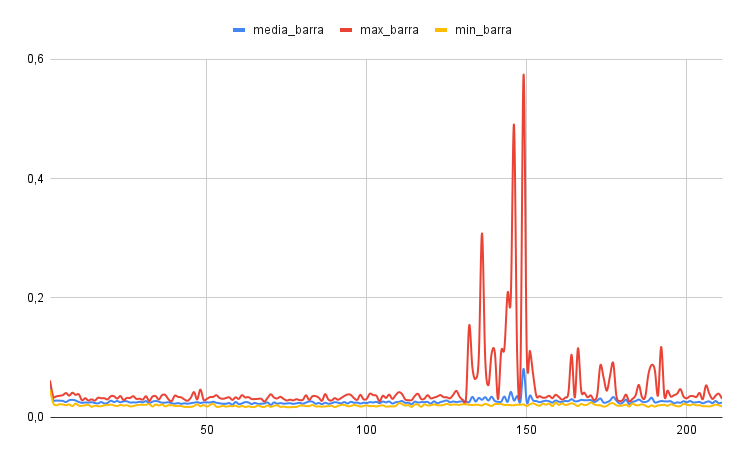
\includegraphics[scale=0.5]{figuras/grafico/barra.png}
	\legend{Fonte: Elaborado pelo autor (2023)}
\end{figure}

\begin{figure}[H]
	\centering
	\caption{Tempo de execução da função 'verify\_inclination' em 10 iterações mostrando a média, mínimo e máximo do tempo gasto por quadro em segundos}
	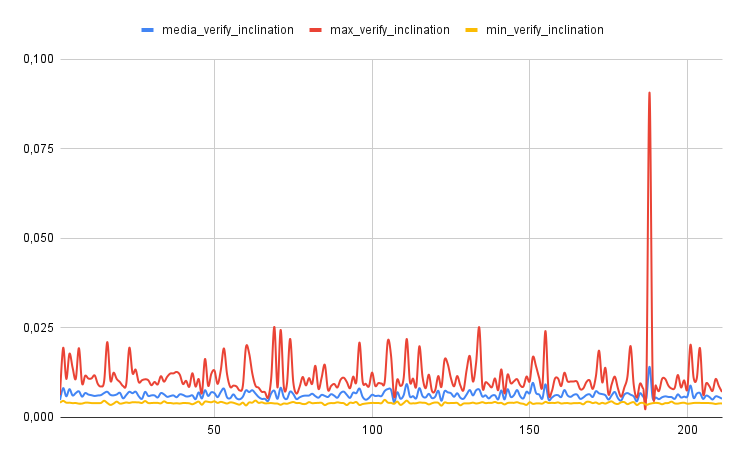
\includegraphics[scale=0.5]{figuras/grafico/inclination.png}
	\legend{Fonte: Elaborado pelo autor (2023)}
\end{figure}


\begin{figure}[H]
	\centering
	\caption{Tempo de execução da função 'verify\_eph' em 10 iterações mostrando a média, mínimo e máximo do tempo gasto por quadro em segundos}
	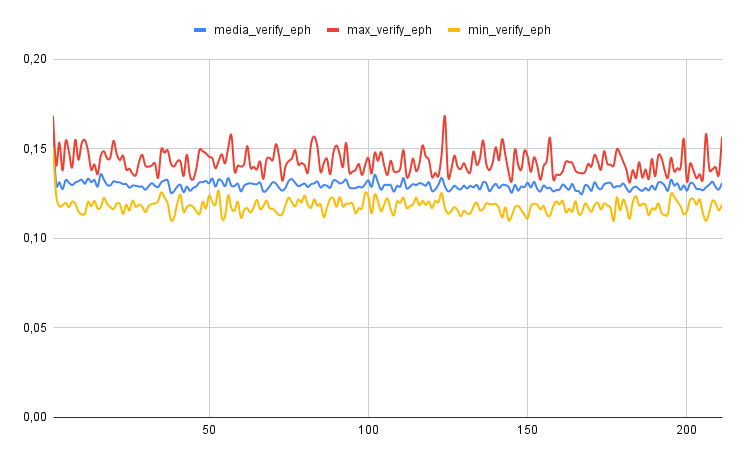
\includegraphics[scale=0.5]{figuras/grafico/eph.png}
	\legend{Fonte: Elaborado pelo autor (2023)}
\end{figure}


\begin{figure}[H]
	\centering
	\caption{Tempo de execução da função 'verify\_angle\_member' em 10 iterações mostrando a média, mínimo e máximo do tempo gasto por quadro em segundos}
	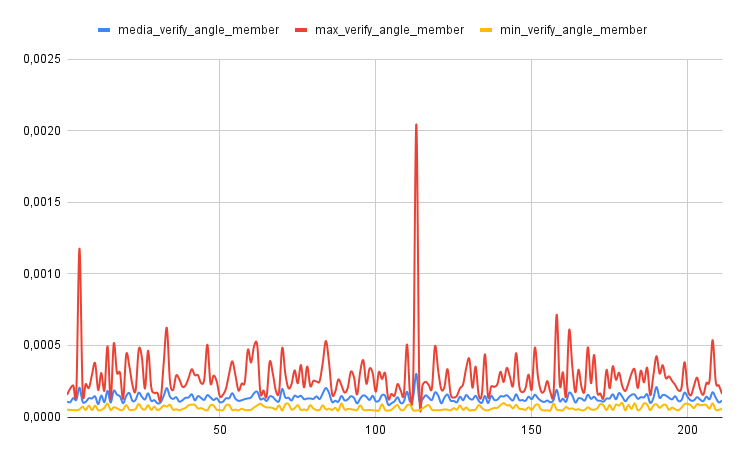
\includegraphics[scale=0.6]{figuras/grafico/angulo.png}
	\legend{Fonte: Elaborado pelo autor (2023)}
\end{figure}


\begin{figure}[H]
	\centering
	\caption{Tempo de execução da função 'verify\_char\_AFD' em 10 iterações mostrando a média, mínimo e máximo do tempo gasto por quadro em segundos}
	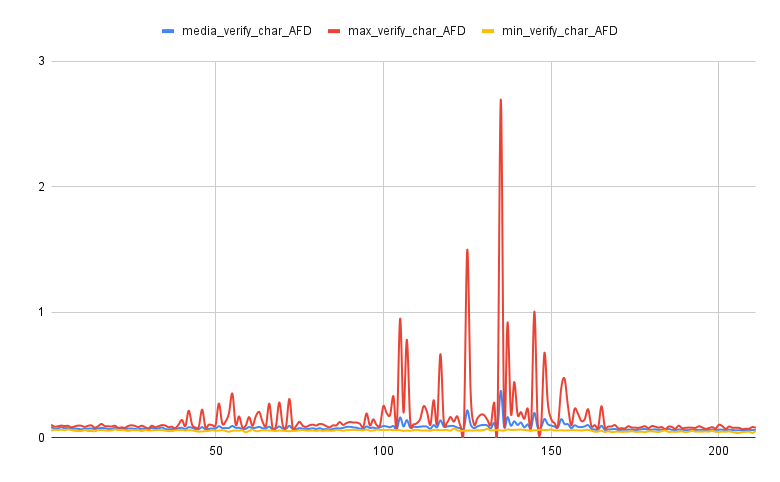
\includegraphics[scale=0.55]{figuras/grafico/char_AFD.png}
	\legend{Fonte: Elaborado pelo autor (2023)}
\end{figure}



\begin{figure}[H]
	\centering
	\caption{Tempo de execução da função 'verify\_maoBarra' em 10 iterações mostrando a média, mínimo e máximo do tempo gasto por quadro em segundos}
	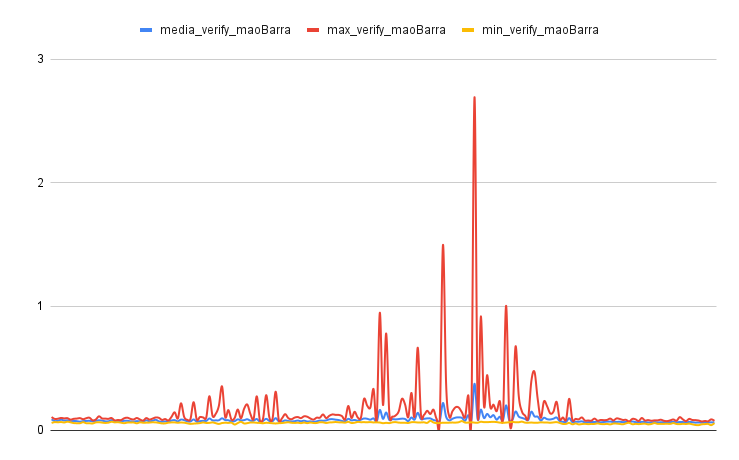
\includegraphics[scale=0.45]{figuras/grafico/maoBarra.png}
	\legend{Fonte: Elaborado pelo autor (2023)}
\end{figure}


\begin{figure}[H]
	\centering
	\caption{Tempo de execução da função 'verify\_extensaoCotovelo' em 10 iterações mostrando a média, mínimo e máximo do tempo gasto por quadro em segundos}
	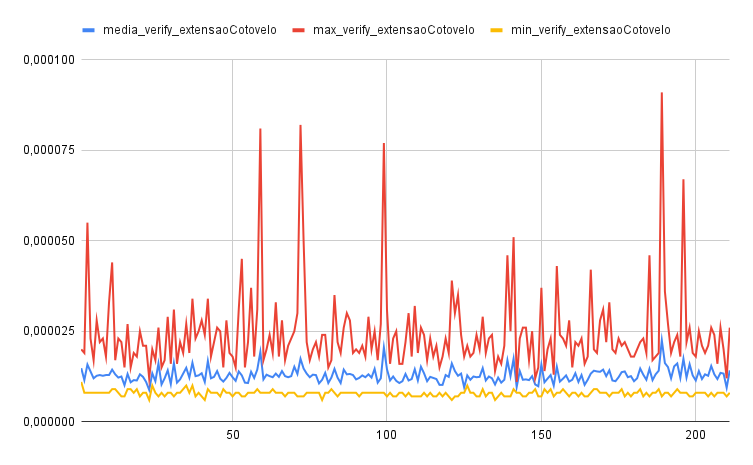
\includegraphics[scale=0.45]{figuras/grafico/extensaoCotovelo.png}
	\legend{Fonte: Elaborado pelo autor (2023)}
\end{figure}


\begin{figure}[H]
	\centering
	\caption{Tempo de execução da função 'verify\_ultrapassarBarra' em 10 iterações mostrando a média, mínimo e máximo do tempo gasto por quadro em segundos}
	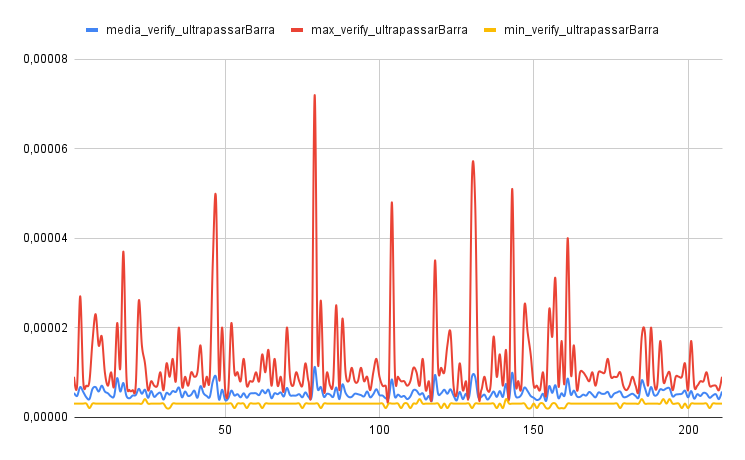
\includegraphics[scale=0.55]{figuras/grafico/ultrapassarBarra.png}
	\legend{Fonte: Elaborado pelo autor (2023)}
\end{figure}


\begin{figure}[H]
	\centering
	\caption{Tempo de execução da função 'verify\_movimentoQuadrilPerna' em 10 iterações mostrando a média, mínimo e máximo do tempo gasto por quadro em segundos}
	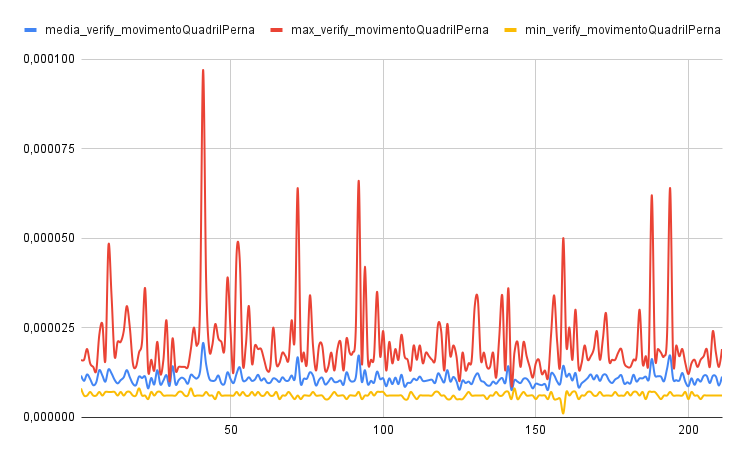
\includegraphics[scale=0.55]{figuras/grafico/movimentoQuadril.png}
	\legend{Fonte: Elaborado pelo autor (2023)}
\end{figure}


\begin{figure}[H]
	\centering
	\caption{Tempo de execução da função 'verify\_AFD' em 10 iterações mostrando a média, mínimo e máximo do tempo gasto por quadro em segundos}
	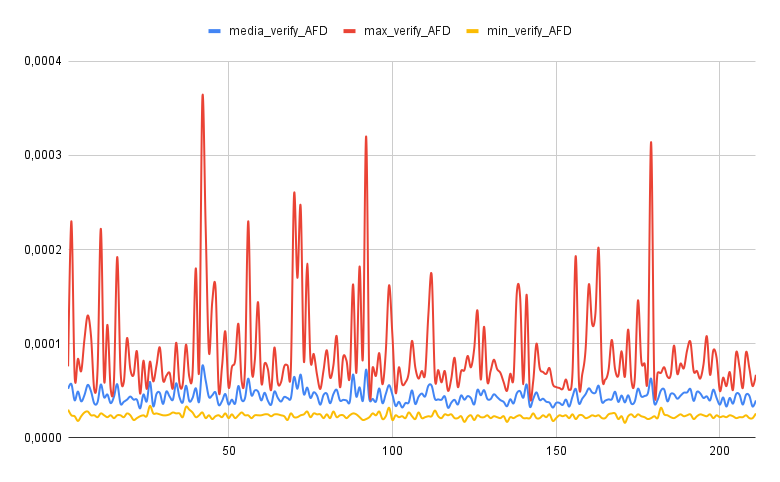
\includegraphics[scale=0.55]{figuras/grafico/verify_AFD.png}
	\legend{Fonte: Elaborado pelo autor (2023)}
\end{figure}


\begin{figure}[H]
	\centering
	\caption{Tempo de execução da função 'process\_cell' em 10 iterações mostrando a média, mínimo e máximo do tempo gasto por quadro em segundos}
	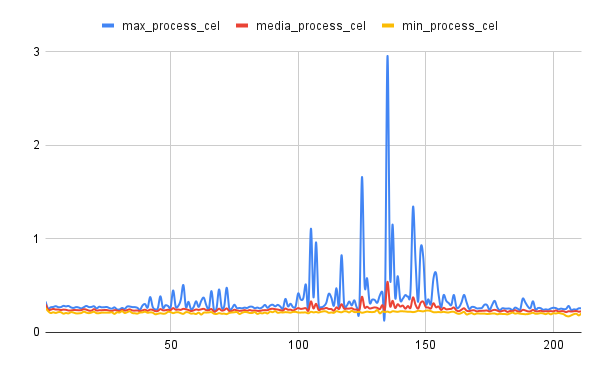
\includegraphics[scale=0.8]{figuras/grafico/process_cell.png}
	\legend{Fonte: Elaborado pelo autor (2023)}
\end{figure}










\newpage

O gráfico a seguir mostra o desempenho relativo de cada função que compõe 'verify\_char\_AFD' em relação a propria função 'verify\_char\_AFD'

\begin{figure}[H]
	\centering
	\caption{ Média de 10 iterações do percentual de tempo gasto por cada função que compõe 'verify\_char\_AFD' }
	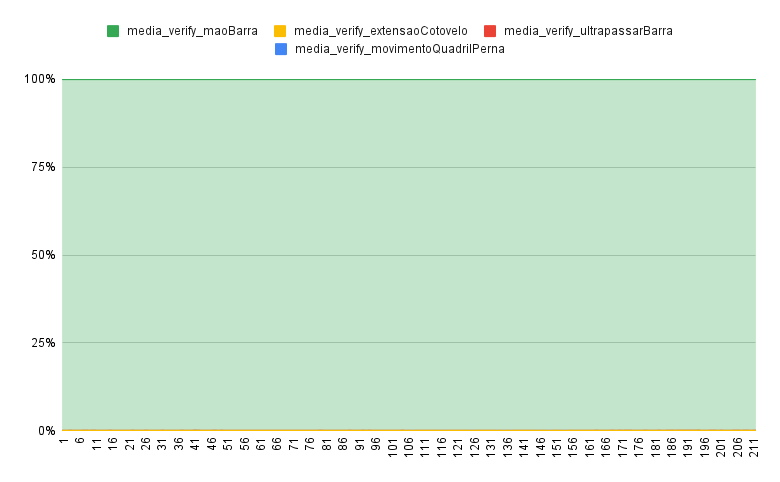
\includegraphics[scale=0.6]{figuras/grafico/comp_char_AFD.png}
	\legend{Fonte: Elaborado pelo autor (2023)}
\end{figure}




O gráfico a seguir apresenta, com base em 10 iterações, a média do tempo gasto em segundos por cada função que compõe 'process\_cell'.

\begin{figure}[H]
	\centering
	\caption{Tempo médio de execução das funções que compõe 'process\_cell'}
	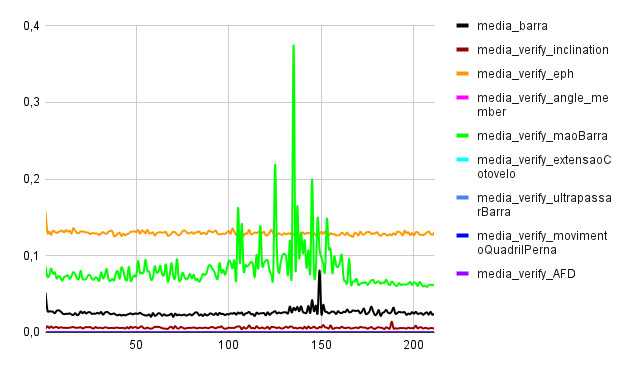
\includegraphics[scale=0.7]{figuras/grafico/comp_process_cell_2.png}
	\legend{Fonte: Elaborado pelo autor (2023)}
\end{figure}


O gráfico a seguir mostra o desempenho relativo de cada função que compõe 'process\_cell' em relação a propria função 'process\_cell'

\begin{figure}[H]
	\centering
	\caption{Média de 10 iterações do percentual de tempo gasto por cada função associado ao processamento de um frame}
	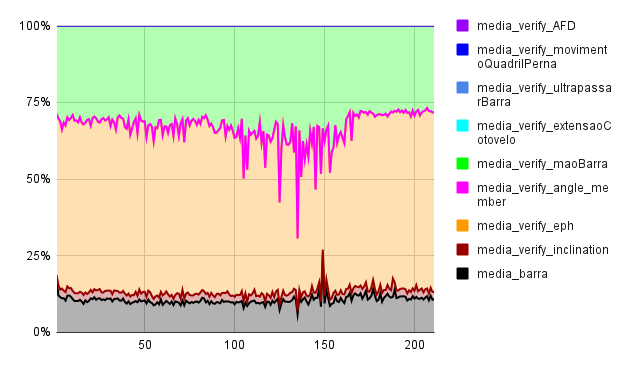
\includegraphics[scale=0.7]{figuras/grafico/comp_process_cell_1.png}
	\legend{Fonte: Elaborado pelo autor (2023)}
\end{figure}






As 2 funções mais relevantes para a alta taxa de latência do processamento do frame são 'verify\_eph' e 'verify\_maoBarra' sendo responsavel por cerca de 85.14\% do tempo gasto por 'process\_cell'



\begin{table}[h]
	\centering
	\begin{tabular}{|p{6cm}|p{3cm}|p{5cm}|}
	\hline
	\textbf{Função} & \textbf{Tempo médio em segundos} & \textbf{Menor tempo registrado em segundos} \\
	\hline
	barra & 0,03422 & 0,016335 \\
	verify\_inclination & 0,00603 & 0,00317 \\
	verify\_eph & 0,1293617 & 0,109623 \\
	verify\_angle\_member & 0,00013 & 0,000045 \\
	verify\_char\_AFD & 0,0753571 & 0,039386 \\
	verify\_AFD & 0,0000427 & 0,000016 \\
	\hline
	\end{tabular}
	\caption{Tempos médios e menores tempos registrados para cada função que compõe process\_cell}
	\label{tab:tempos_funcoes}
\end{table}



\begin{table}[h]
	\centering
	\begin{tabular}{|p{6cm}|p{3cm}|p{5cm}|}
	\hline
	\textbf{Função} & \textbf{Tempo médio em segundos} & \textbf{Menor tempo registrado em segundos} \\
	\hline
	verify\_maoBarra & 0,0747025 & 0,03924 \\
	verify\_extensaoCotovelo & 0,0000126 & 0,000006  \\
	verify\_ultrapassarBarra & 0,0000051 & 0,000002  \\
	verify\_movimentoQuadrilPerna & 0,0000104 & 0,000001  \\
	\hline
	\end{tabular}
	\caption{Tempos médios e menores tempos registrados para cada função que compõe verify\_char\_AFD}
	\label{tab:tempos_funcoes_especificas}
\end{table}
	
Por fim  o tempo médio para a execução da função 'process\_cell' foi de 0,2481895403 segundos, enquanto o menor tempo registrado foi de 0,171841 segundos assumindo um desvio padrão de 0,03161229806 e uma variancia de 0,0009993373889.

